%!TEX root = ../thesis.tex


\ifpdf
    \graphicspath{{Appendix1/Figs/Raster/}{Appendix1/Figs/PDF/}{Appendix1/Figs/}{Appendix1/}}
\else
    \graphicspath{{Appendix1/Figs/Vector/}{Appendix1/Figs/}{Appendix1/}}
\fi
% ******************************* Thesis Appendix A ****************************
\chapter{Fermion-to-Qubit Mappings} 
\section{Hybrid Mappings}
\subsection{Steiner Tree Solver}
\label{section:SCIPJACK}
In our analysis we evaluate the performance of different mappings on a square-lattice qubit architecture. Some mappings require 2-qubit gates to be performed on non-neighbouring qubits and so we need additional SWAP gates. Calculating the optimum choice of SWAP gates requires finding the minimum path length required to connect all the qubits involved in a given fermionic operation. This is an example of an NP-hard problem known as the Steiner Tree problem:

\begin{algorithm}[h]
\centering
\caption*{\label{alg:steinerTree}\textsc{Steiner Tree Problem}}
\begin{algorithmic}
\State \textsc{Given an undirected connected graph $G = (V,E)$ and a set $T \in V$ of terminals, find a tree $S \in G$ of minimum length that spans $T$}
\end{algorithmic}
\end{algorithm}

In our case the set of terminals corresponds to the set of qubits involved in the given fermionic operation which we want to find the minimum path of SWAP gates between. In our calculations we use a top-ranking Steiner Tree solver SCIP-JACK \cite{rehfeldt2021implications} to find this minimum path.  SCIP-JACK consists of three component parts: preprocessing, primal heuristics, and a branch-and-cut procedure.

The preprocessing uses reduction techniques to reduce the size of the graph whilst still allowing at least one solution to the reduced problem to be converted into an optimal solution to the original graph. Examples of these techniques include merging together connected vertices that share no other neighbours or discarding 1-degree non-terminal vertices.

The primal heuristic finds good or optimal solutions to the problem. In SCIP-JACK the one-phase repetitive shortest path heuristic \cite{aragao2002implementation} is used. This starts from a vertex and uses Dijkstra’s algorithm \cite{dijkstra2022note} to find the shortest path to the nearest terminal. This procedure is then reiterated with the modification to Dijkstra’s algorithm that the tentative distance assigned to each vertex is carried over. Once this has built up a subgraph containing all the terminals, a minimum spanning tree is constructed covering the subgraph, and any 1-degree non-terminal vertices are pruned.

The branch-and-cut procedure is the backbone of the program used to compute a lower bound and prove the optimality of the solution. First, the problem is expressed in terms of a integer programming problem by considering $x_e$ to be binary variables representing whether edge $e \in E$ is included in the Steiner tree:

\begin{algorithm}
\centering
\caption*{\label{alg:steinerTreeCut}\textsc{Steiner Tree Problem Undirected Cut Formulation}}
\begin{minipage}{.4\linewidth}
\begin{algorithmic}[1]
\Statex Define $\delta (U) =\{\{u,v\} \in E: u \in U, v \in V/U \}$
\Statex
\Statex Find min $\sum_e x_e$ under the following constraints:
\State $x(\delta (W)) \geq 1$ for all $W \in V$, $0 < |W \cap T| < |T|$
\State $x_e \in \{0,1\} \forall e \in E$
\end{algorithmic}
\end{minipage}
\end{algorithm}

Linear programming is used to initially optimise the solution when considering only a subset of these constraints providing a lower bound on an optimal solution. The primary heuristic is then run with edge costs given by $1-x_e$ to find a feasible solution (reasonably similar to the LP solution) providing an upper bound on the optimal solution. Then, the algorithm considers the restraints ("cuts") that the current solution violates and adds them to the subset of constraints in the linear programming model. This model is repeatedly solved and expanded until the subset of constraints has grown sufficiently. At this point, if the solution is integral then we have found an optimal solution, otherwise the algorithm "branches" by creating two new sub-problems (nodes) each with an additional constraint on one of the variables ($x_e$) that forces it to be either 0 or 1 in each problem respectively. The process is then repeated again on each of these nodes (potentially with more constraints added). If for any node the optimal solution exceeds any of the heuristic solutions found, the node is discarded (pruned).
\newpage
\subsection{Visual guide to Hybrid mappings}
In this section we provide a series of diagrams to further elaborate and explain our hybrid mapping algorithms.\\\\
Figures~\ref{ZPattern} and \ref{SPattern} respectively describe the Jordan-Wigner mapping over the roots of Bravyi-Kitaev cells in the Hybrid and Hybrid\+ mapping schemes.\\\\
Figure~\ref{fig:stabilisers} illustrates the family of stabilisers utilised by the Hybrid\+ mapping scheme. This is identical to the stabilisers found in \cite{steudtner2019quantum}.\\\\
Figures~\ref{fig:verticalInteractionYodd} and \ref{fig:horizontalInteractionXYYX} demonstrate how the Hybrid\+ mapping scheme shortens different Pauli-strings.\\\\
In the figures below: the dashed boxes represent the cells, whilst the circles inside them represent the roots of each cell, and the circles without boxes represent the ancillas.
\renewcommand\thefigure{\thesection.\arabic{figure}}
\setcounter{figure}{0}    
\label{appendix}
    \begin{figure}[h]
    \begin{minipage}{0.5\textwidth}
        \centering
         \includegraphics[page=20, width=\textwidth  , height=5.75cm]{Hybrid_Fermion_Mapping_diagrams.pdf}
        \caption{ \label{ZPattern}Diagram illustrating how the \textit{cell number} is assigned in a Z pattern to each cell in the Hybrid mapping.}
        \end{minipage}%
        \begin{minipage}{0.5\textwidth}
        \centering
         \includegraphics[page=19, width=\textwidth  , height=5.75cm]{Hybrid_Fermion_Mapping_diagrams.pdf}
        \caption{\label{SPattern}Diagram illustrating how the \textit{cell number} is assigned in a S pattern to each cell in the Hybrid\+ mapping. The unnumbered circles represent the ancillas each connected to the cell directly below them.}
        \end{minipage}
    \end{figure}
            \begin{figure*}[btp]
        \centering
        \begin{subfigure}{.5\textwidth}
        \includegraphics[page=2, width=\textwidth  , height=6cm]{Hybrid_Fermion_Mapping_diagrams.pdf}
        \end{subfigure}%
        \begin{subfigure}{.5\textwidth}
        \includegraphics[page=3, width=\textwidth  , height=6cm]{Hybrid_Fermion_Mapping_diagrams.pdf}
        \end{subfigure}%
        
                \caption{\label{fig:stabilisers} Examples from the family of stabilisers created by applying the series of gates illustrated in \ref{fig:entangleEdge} and \ref{fig:entangleRow}. The family consists of a stabiliser for every ancilla which is a string of Z gates that follow the line of the S-pattern with either $XXY$ or $YXX$ gates surrounding the ancilla depending on whether the row is odd or even.}
    \end{figure*}
       \begin{figure*}
       \begin{minipage}{\textwidth}
           \begin{minipage}{0.5\textwidth}
        \includegraphics[page=9, width=\textwidth  , height=5.75cm]{Hybrid_Fermion_Mapping_diagrams.pdf}
        \tikz[baseline=-\baselineskip]\draw[ultra thick,->] (0,0) -- ++ (0,-0.5);
        \includegraphics[page=10, width=\textwidth  , height=5.75cm]{Hybrid_Fermion_Mapping_diagrams.pdf}
        \end{minipage}%
    \begin{minipage}{0.5\textwidth}
        \includegraphics[page=11, width=\textwidth  , height=5.75cm]{Hybrid_Fermion_Mapping_diagrams.pdf}
        \tikz[baseline=-\baselineskip]\draw[ultra thick,->] (0,0) -- ++ (0,-0.5);
        \includegraphics[page=12, width=\textwidth  , height=5.75cm]{Hybrid_Fermion_Mapping_diagrams.pdf}
        \end{minipage}
        \begin{minipage}{0.5\textwidth}
        \includegraphics[page=13, width=\textwidth  , height=5.75cm]{Hybrid_Fermion_Mapping_diagrams.pdf}
        \tikz[baseline=-\baselineskip]\draw[ultra thick,->] (0,0) -- ++ (0,-0.5);
        \includegraphics[page=14, width=\textwidth  , height=5.75cm]{Hybrid_Fermion_Mapping_diagrams.pdf}
\end{minipage}%
        \begin{minipage}{0.5\textwidth}
        \includegraphics[page=15, width=\textwidth  , height=5.75cm]{Hybrid_Fermion_Mapping_diagrams.pdf}
        \tikz[baseline=-\baselineskip]\draw[ultra thick,->] (0,0) -- ++ (0,-0.5);
        \includegraphics[page=16, width=\textwidth , height=5.75cm]{Hybrid_Fermion_Mapping_diagrams.pdf}
\end{minipage}
\end{minipage}
        \caption{\label{fig:verticalInteractionYodd}Diagrams showing how the portion of Pauli-strings acting on the roots of cells are modified and simplified by the Hybrid\+ mapping algorithm}
    \end{figure*}
\begin{figure}
\centering
 \begin{minipage}{0.5\textwidth}
        \includegraphics[page=17, width=\textwidth  , height=6cm]{Hybrid_Fermion_Mapping_diagrams.pdf}
        \tikz[baseline=-\baselineskip]\draw[ultra thick,->] (0,0) -- ++ (0,-0.5);
        \includegraphics[page=18, width=\textwidth  , height=6cm]{Hybrid_Fermion_Mapping_diagrams.pdf}
        \end{minipage}
        \caption{\label{fig:horizontalInteractionXYYX}Diagrams showing how the portion of a Pauli-string acting on the roots of the cells is modified and simplified by the Hybrid\+ mapping algorithm}
    \end{figure}